% (The MIT License)
%
% Copyright (c) 2023-2024 Yegor Bugayenko
%
% Permission is hereby granted, free of charge, to any person obtaining a copy
% of this software and associated documentation files (the 'Software'), to deal
% in the Software without restriction, including without limitation the rights
% to use, copy, modify, merge, publish, distribute, sublicense, and/or sell
% copies of the Software, and to permit persons to whom the Software is
% furnished to do so, subject to the following conditions:
%
% The above copyright notice and this permission notice shall be included in all
% copies or substantial portions of the Software.
%
% THE SOFTWARE IS PROVIDED 'AS IS', WITHOUT WARRANTY OF ANY KIND, EXPRESS OR
% IMPLIED, INCLUDING BUT NOT LIMITED TO THE WARRANTIES OF MERCHANTABILITY,
% FITNESS FOR A PARTICULAR PURPOSE AND NONINFRINGEMENT. IN NO EVENT SHALL THE
% AUTHORS OR COPYRIGHT HOLDERS BE LIABLE FOR ANY CLAIM, DAMAGES OR OTHER
% LIABILITY, WHETHER IN AN ACTION OF CONTRACT, TORT OR OTHERWISE, ARISING FROM,
% OUT OF OR IN CONNECTION WITH THE SOFTWARE OR THE USE OR OTHER DEALINGS IN THE
% SOFTWARE.

\documentclass{article}
\usepackage{../sqm}
\newcommand*\thetitle{Comments Density}
\begin{document}

\plush{\sqmTitlePage{19}{}}

\qte
  [Brian Kernighan]
  {brian-kernighan.jpg}
  {The best documentation for a computer program is a \ul{clean structure}. It also helps if the code is well formatted, with good mnemonic identifiers, labels, and a smattering of \ul{enlightening comments}. Flowcharts and program descriptions are of secondary importance; the only reliable documentation of a computer program is the \ul{code} itself.}
  {kernighan1974elements}

\pitch{\begin{multicols}{2}
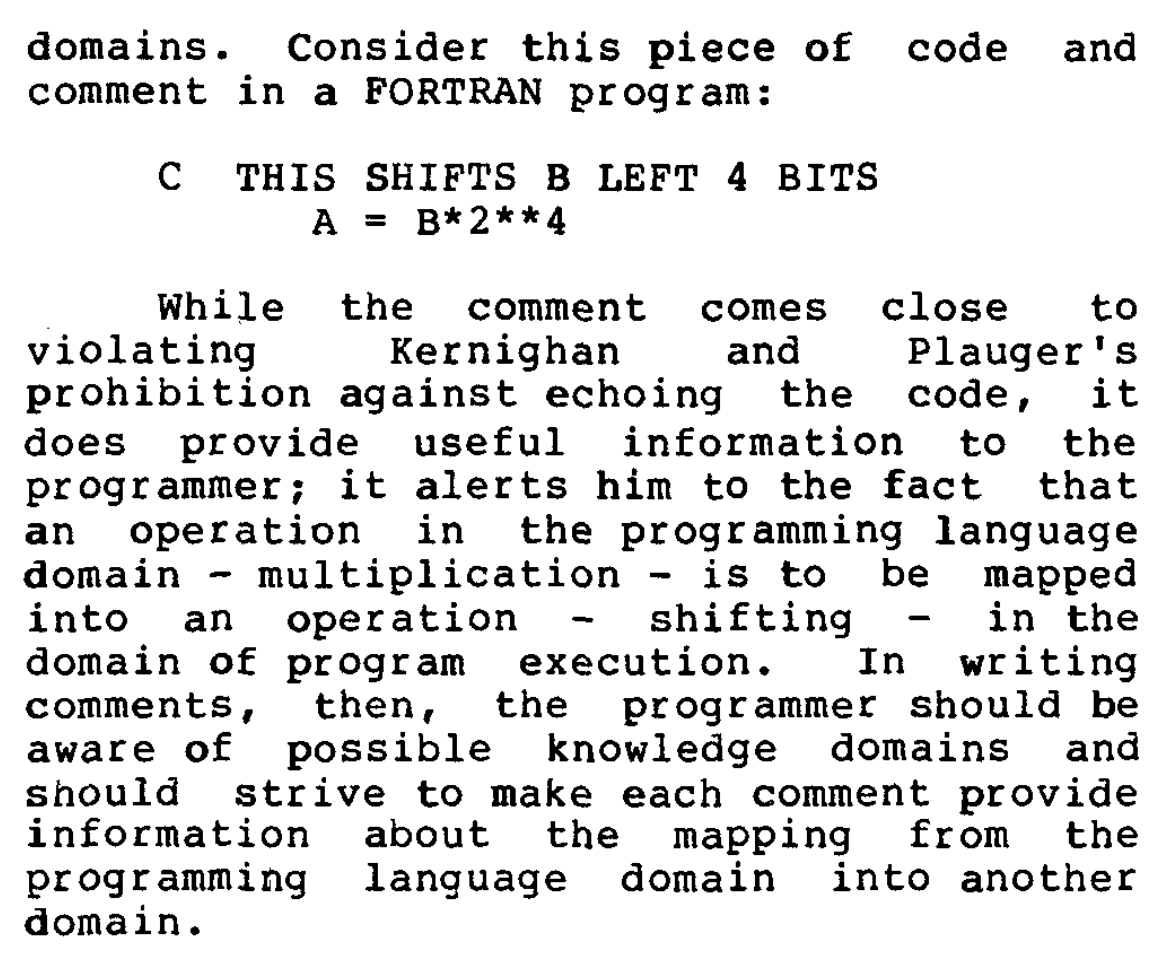
\includegraphics[width=\linewidth]{bridge.png}
\par\columnbreak\par
``Comments which precede a group of statements, and which describe them in terms of operations in another domain, will be particularly helpful. The role of comments is to \ul{bridge} between knowledge domains.''
\source{brooks1978using}
\end{multicols}}

\qte
  [Hubert E. Dunsmore]
  {hubert-dunsmore.jpg}
  {An experiment was conducted to investigate how comments are related to programmers' ability to \ul{understand} programs. Those programmers whose programs contained comments were able to \ul{answer} more questions than those without comments.}
  {woodfield1981effect}

\qte
  {../05-maintainability-index/paper-1.png}
  {[The degree of] \ul{intramodule commenting} is the number of lines with comments divided by the total number of lines in the module, averaged over all modules.}
  {oman1992metrics}

\qte
  [David Parnas]
  {david-parnas.jpg}
  {Documentation that seems \ul{clear} and \ul{adequate} to its authors is often about \ul{as clear as mud} to the programmer who must maintain the code six months or \ul{six years later}.}
  {parnas1994software}

\pitch{
\pptBanner{Comments Affect Maintainability}
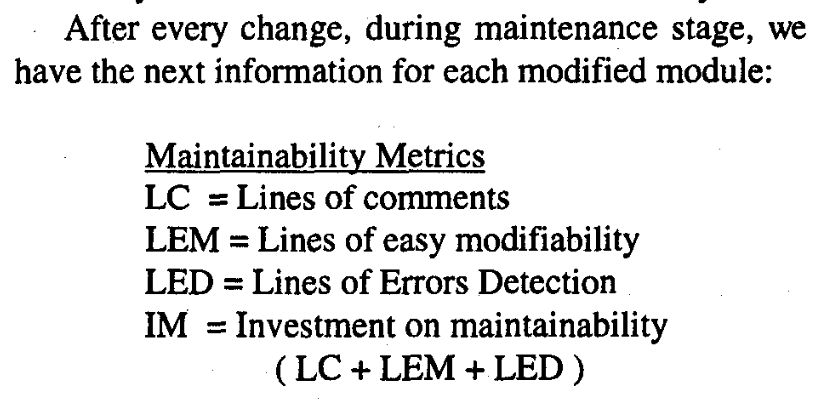
\includegraphics[width=.75\linewidth]{maintainability.png}
\source{garcia1996maintainability}}

\qte
  [Martin Fowler]
  {../06-coupling/martin-fowler.jpg}
  {Don't worry, we aren't saying that people shouldn't write comments. In our olfactory analogy, comments aren't a bad smell; indeed they are a \ul{sweet smell}. The reason we mention comments here is that comments often are used as a \ul{deodorant}. It's surprising how often you look at thickly commented code and notice that the comments are there because the code is bad.}
  {fowler1999refactoring}

\qte
  [Andy Hunt]
  {../11-clone-coverage/andy-hunt.jpg}
  {Programmers are taught: good code has \ul{lots of comments}. Unfortunately, they are never taught why code needs comments: bad code requires lots of comments. The DRY principle tells us to keep the low-level knowledge in the code, where it belongs, and reserve the comments for other, \ul{high-level explanations}. Otherwise, we're duplicating knowledge, and every change means changing both the code and the comments. The comments will inevitably become \ul{out of date}, and untrustworthy comments are worse than no comments at all.}
  {hunt1999pragmatic}

\qte
  [Eriko Nurvitadhi]
  {eriko-nurvitadhi.jpg}
  {The results indicated that method comments do increase \ul{low-level} program understanding, while class comments did not increase \ul{high-level} understanding. This raises questions about the role of class comments in Object-Oriented programs...}
  {nurvitadhi2003class}

\qte
  [Steve McConnell]
  {../06-coupling/steve-mcconnell.jpg}
  {The main contributor to code-level documentation isn't comments, but good \ul{programming style}... Comments are easier to write poorly than well, and commenting can be more \ul{damaging} than helpful.}
  {mcconnell2004code}

\qte
  [Beat Fluri]
  {beat-fluri.jpg}
  {Code and comments \ul{rarely} co-evolve: despite its growth rate, newly added code barely is commented. Also, 97\% of comment changes are done in the same revision as the associated source code change.}
  {fluri2007code}

\qte
  [Robert C. Martin]
  {../09-CAMC-and-NHD/robert-martin.jpg}
  {Indeed, comments are, at best, a \ul{necessary evil}. If our programming languages were expressive enough, or if we had the talent to subtly wield those languages to express our intent, we would not need comments very much---perhaps \ul{not at all}.}
  {martin2008clean}

\qte
  [Oliver Arafat]
  {oliver-arafat.jpg}
  {Comment density is the percentage of comment lines in a given source code base, that is, comment lines divided by total lines of code. Comment density is assumed to be a good \ul{predictor} of maintainability and hence \ul{survival} of a software project. In this study we focus on one particular code metric, the comment density, and assess it across 5,229 active open source projects, representing about 30\% of all active open source projects.}
  {arafat2009comment}

\pitch{
\pptBanner{Project Size vs. Comments Density}
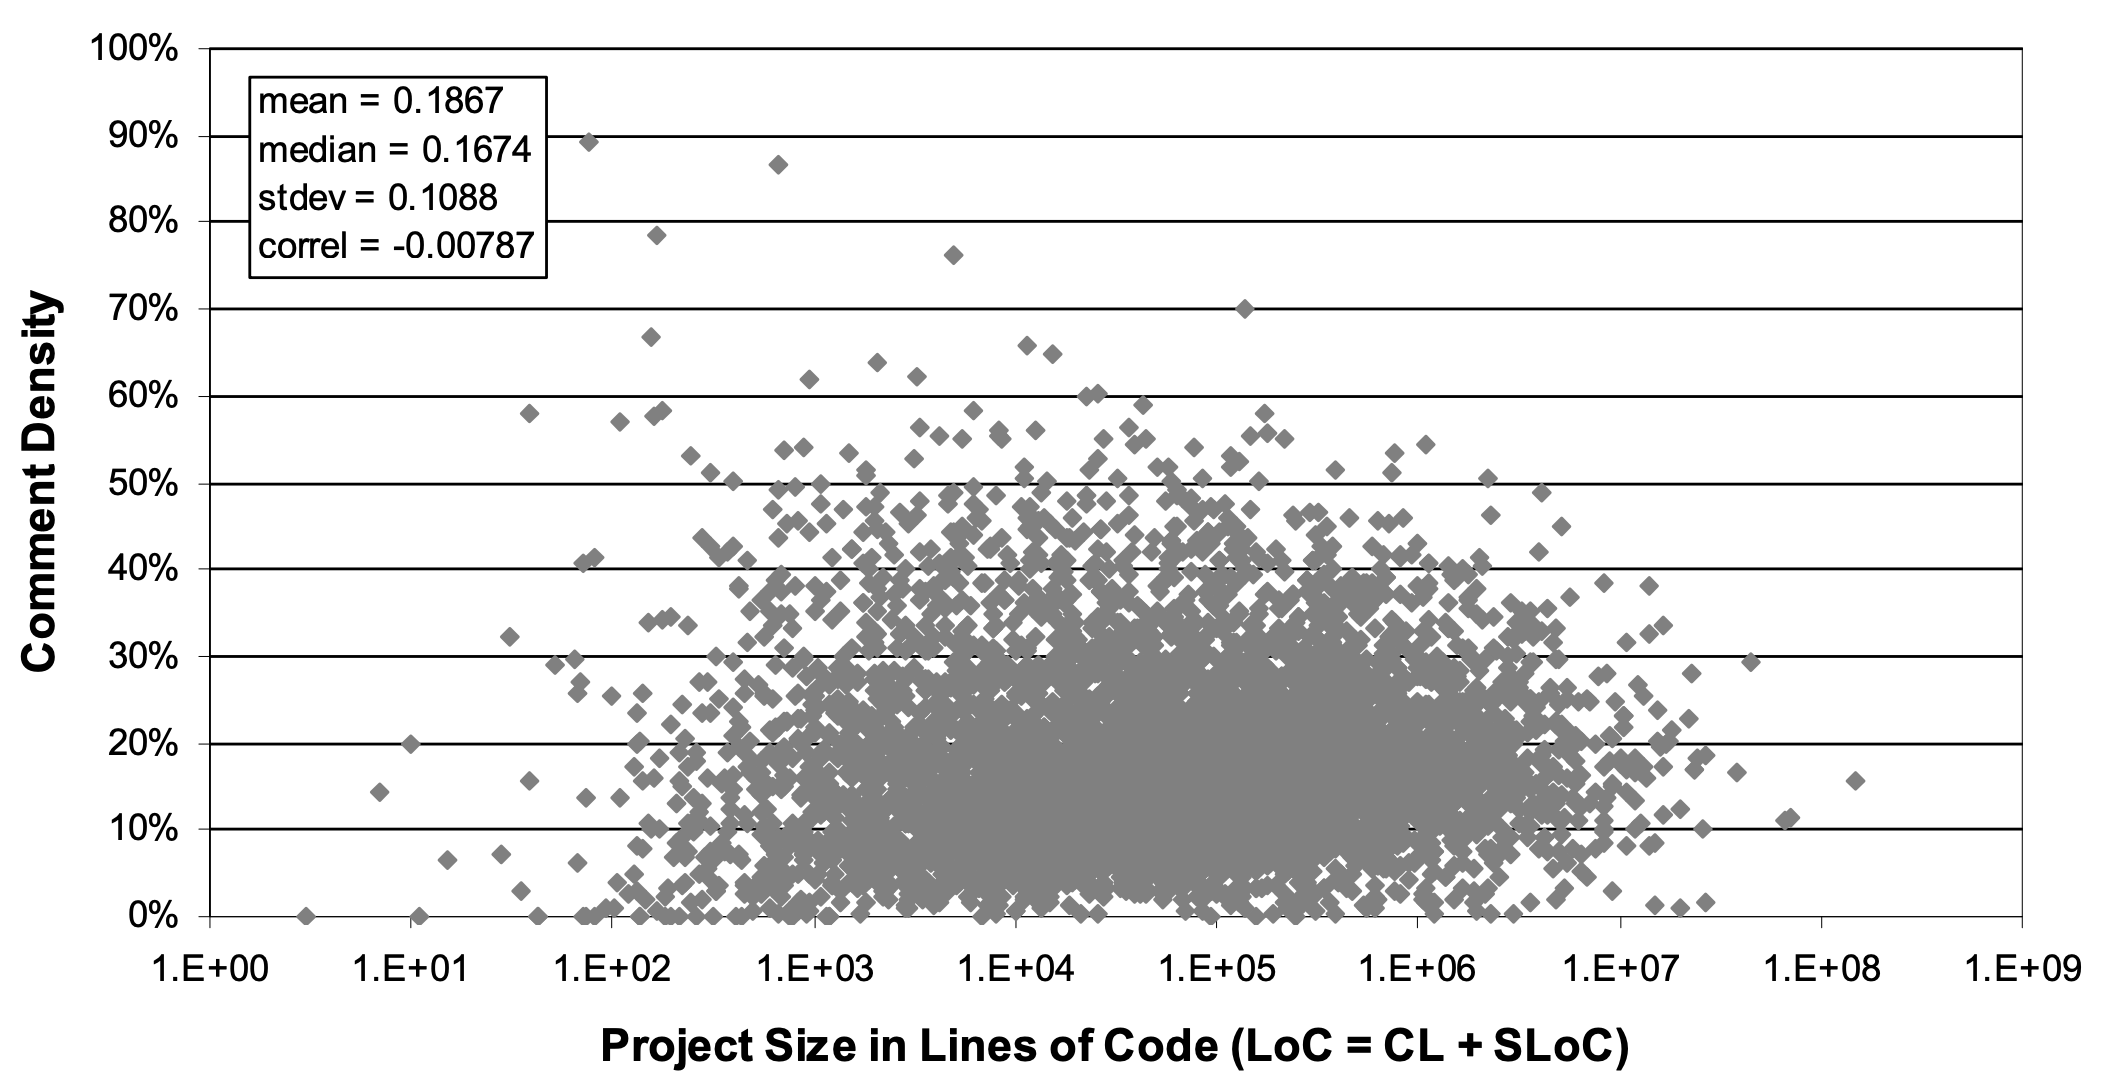
\includegraphics[width=.7\linewidth]{density.png}
\source{arafat2009comment}}

\qte
  [Houari Sahraoui]
  {houari-sahraoui.jpg}
  {We defined a taxonomy of comments to guide this analysis. Our study showed that programmers comment \ul{some constructs} more often than others. In the majority of cases, comments are intended to \ul{explain} the code that follows them. The second more widely used category of comments are dedicated to \ul{communication} between programmers and personal notes (we call them \ul{working} comments).}
  {haouari2011good}

\pitch{
\pptBanner{Types of Comments}
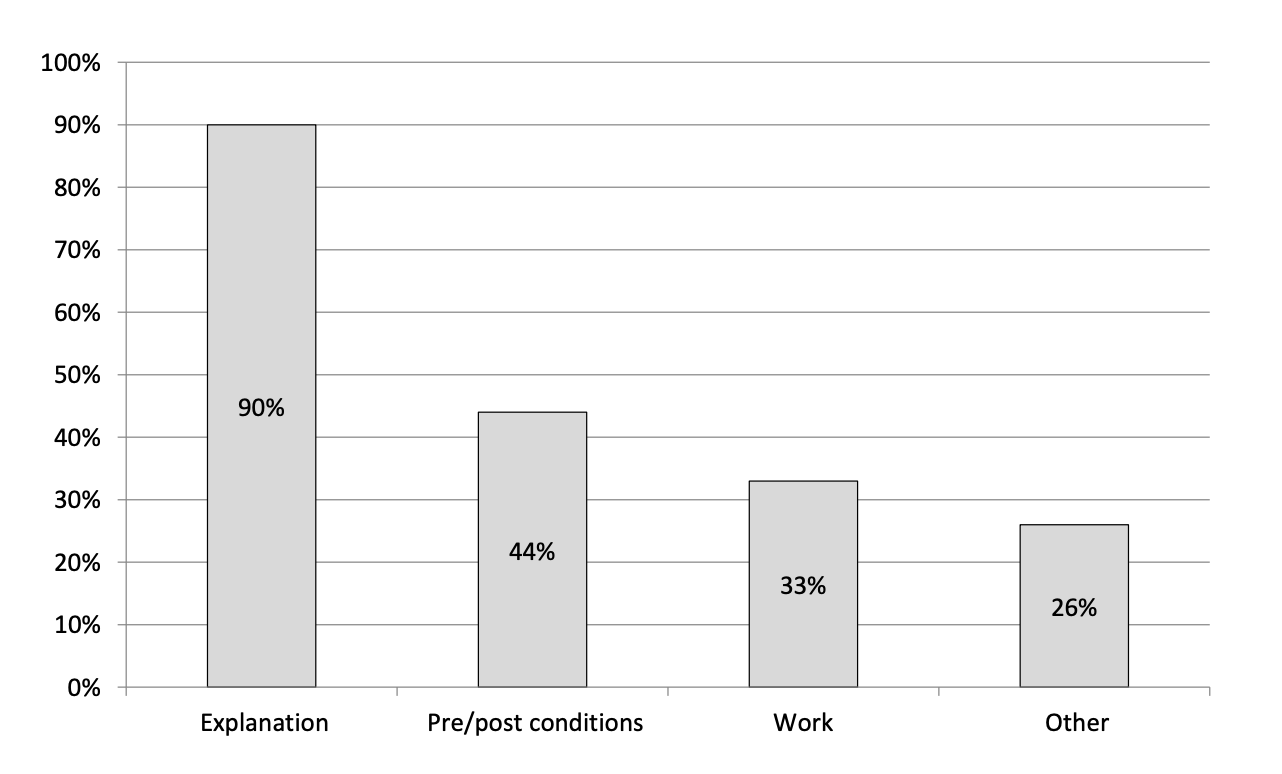
\includegraphics[width=.6\linewidth]{types-of-comments.png}
\source{haouari2011good}}

\pitch{
\pptBanner{Frequency of Comments}
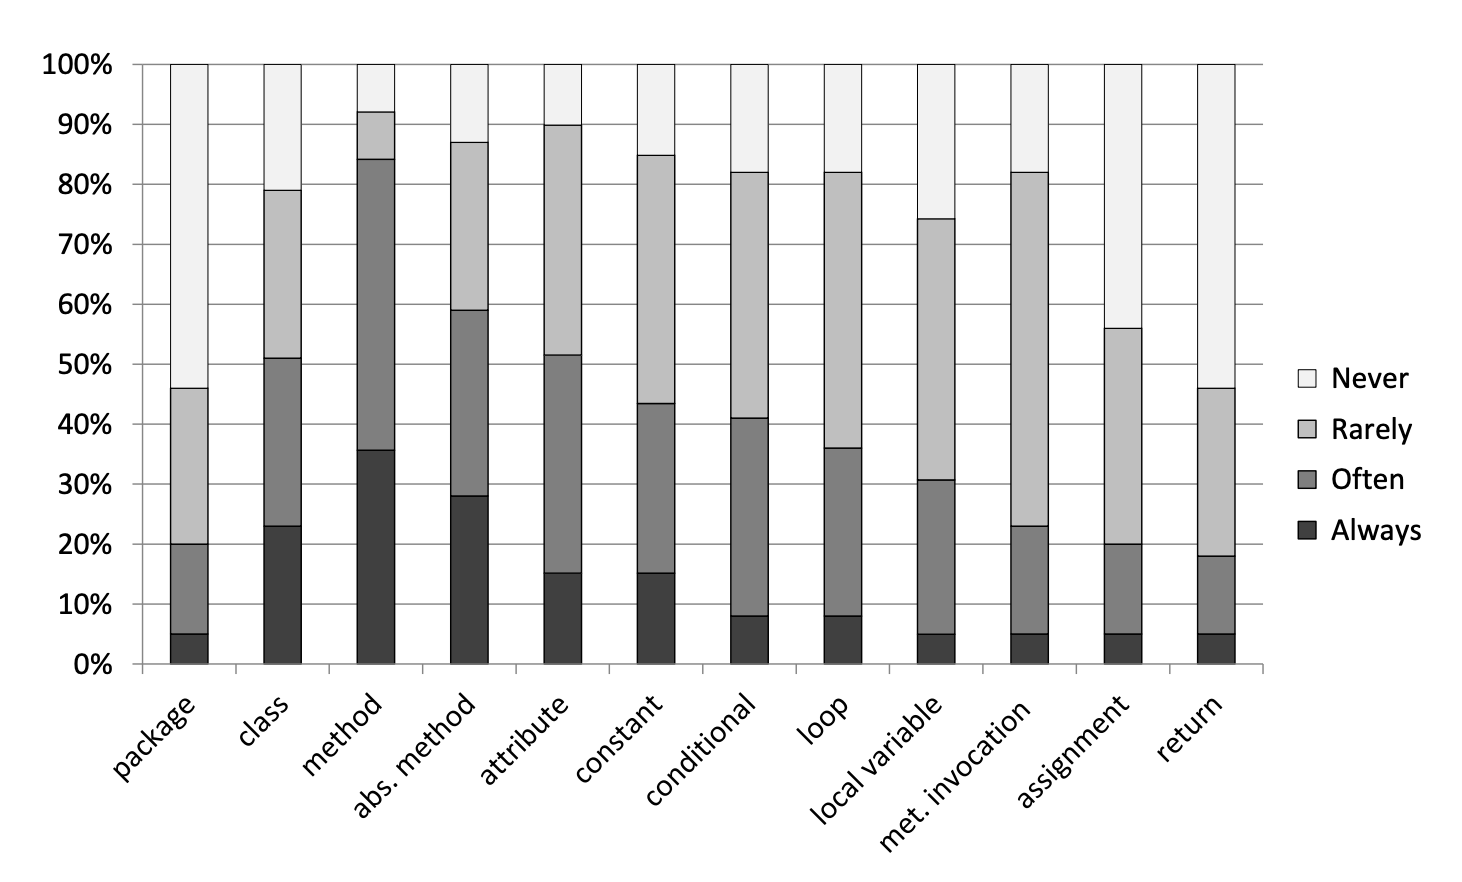
\includegraphics[width=.6\linewidth]{frequency-of-comments.png}
\source{haouari2011good}}

\qte
  [Tobias Röhm]
  {tobias-roehm.jpg}
  {Source code is \ul{more trusted} than documentation: 21 participants reported that they get their main information from \ul{source code} and \ul{inline comments} whereas only four stated that \ul{documentation} is their main source of information.}
  {roehm2012professional}

\qte
  [Luca Pascarella]
  {luca-pascarella.jpg}
  {Code comments contain valuable information to support software development, especially during code reading and code maintenance. Nevertheless, not all the comments are the \ul{same}.}
  {pascarella2019classifying}

\pitch{
\pptBanner{Taxonomy of Comment Types}
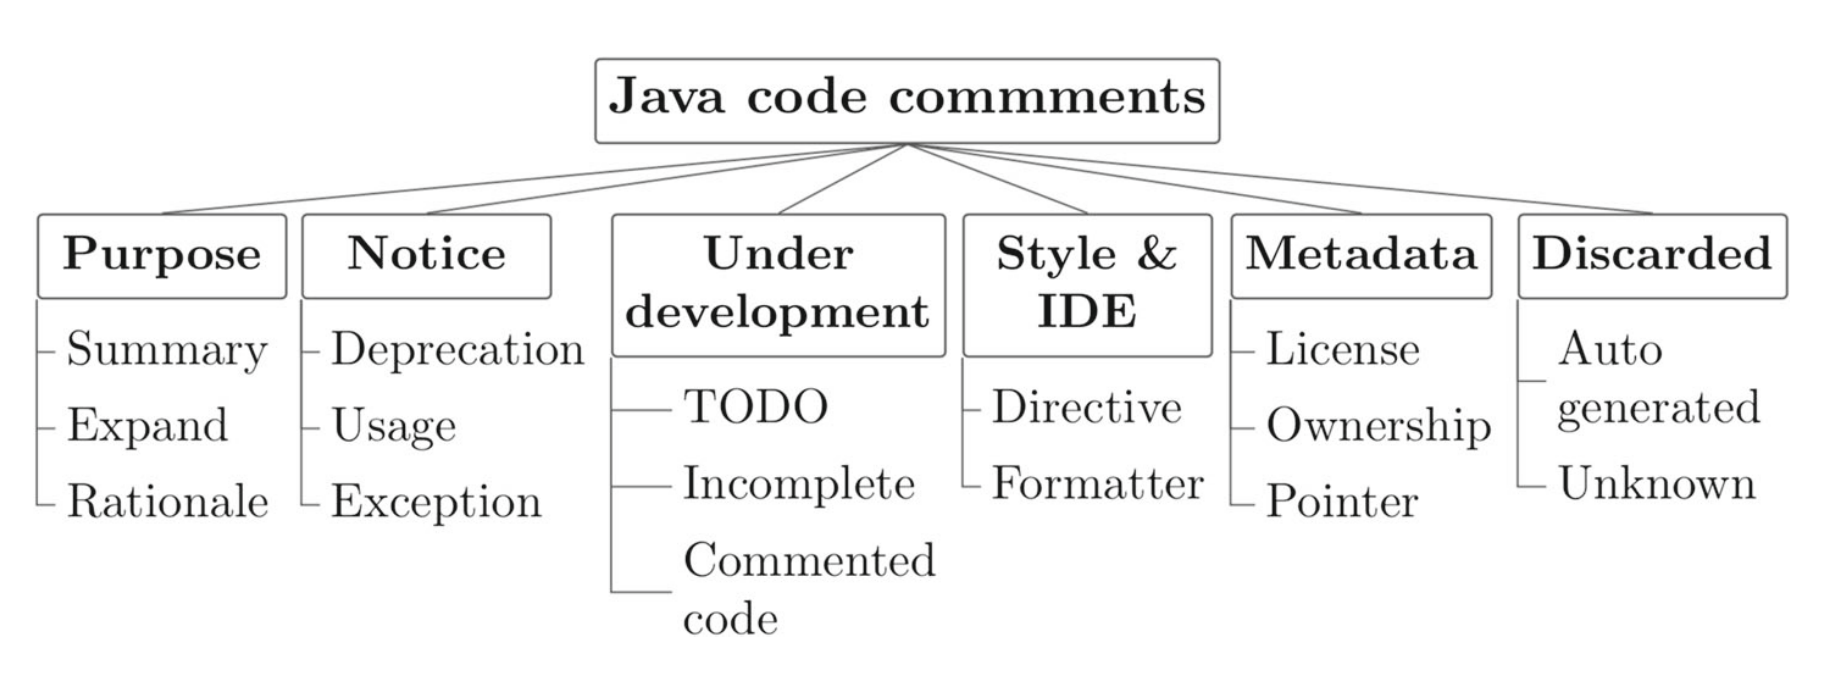
\includegraphics[width=.95\linewidth]{taxonomy.png}
\source{pascarella2019classifying}}

\qte
  [Hao He]
  {hao-he.jpg}
  {We analyzed the comment density of 150 projects in 5 different programming languages. We have found that there are noticeable differences in comment density, which may be related to the \ul{programming language} used in the project and the \ul{purpose} of the project.}
  {he2019understanding}

\pitch{
\pptBanner{Comments Density by Language}
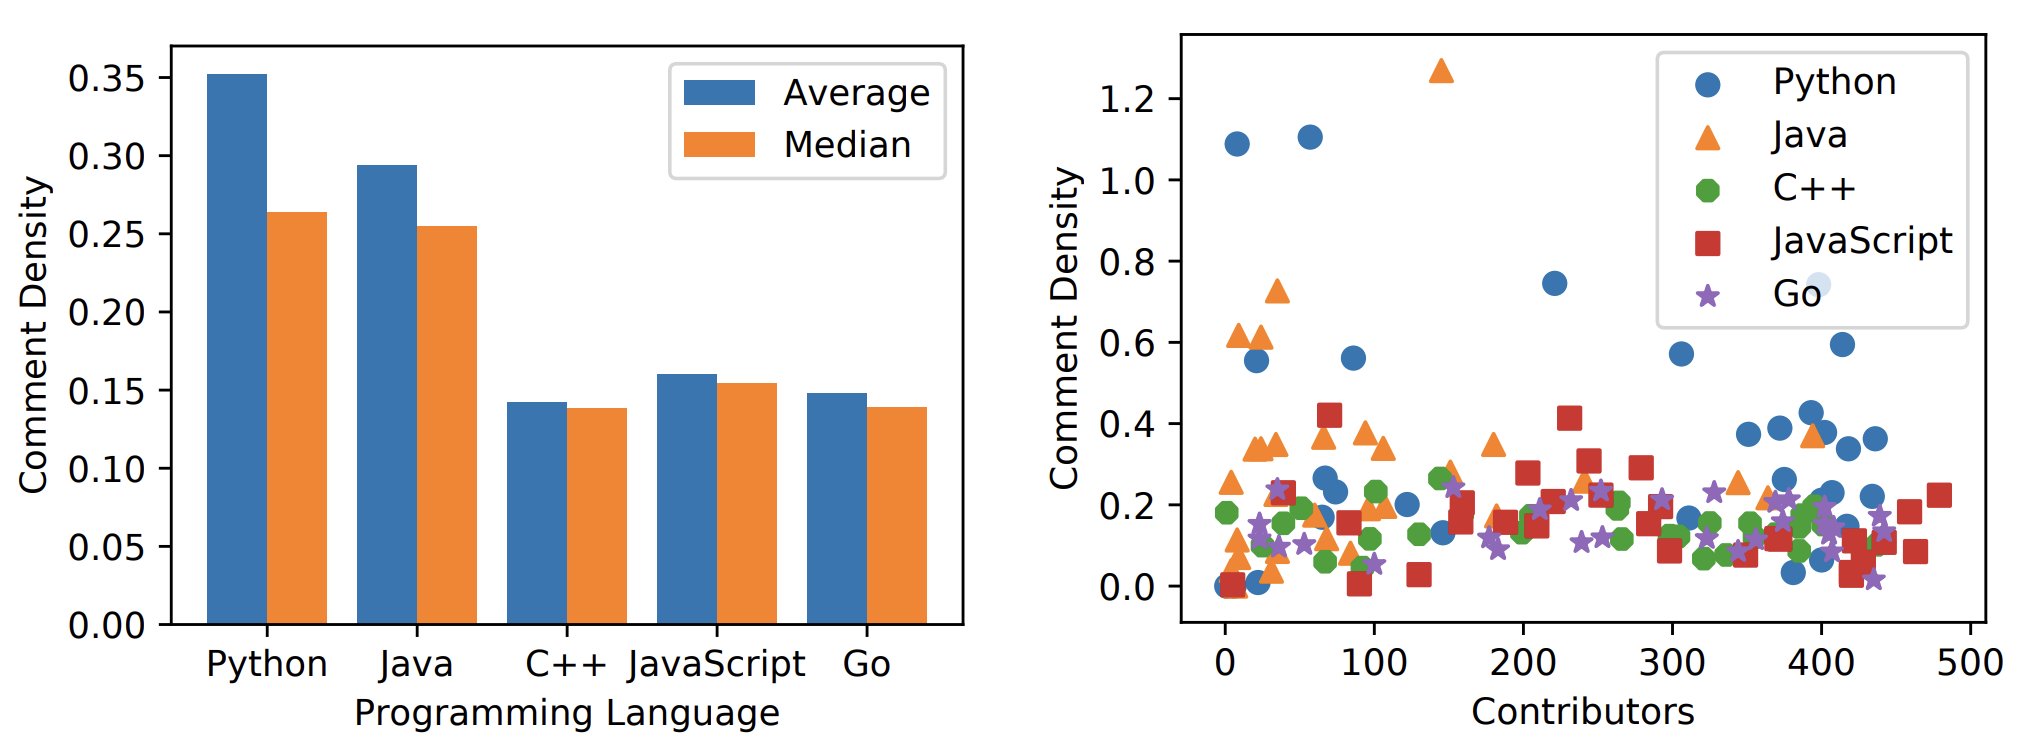
\includegraphics[width=.9\linewidth]{by-language.png}
\source{he2019understanding}}

\qte
  [Sean Stapleton]
  {sean-stapleton.jpg}
  {Participants reviewed Java methods and summaries and answered established program comprehension questions. In addition, participants completed coding tasks given summaries as specifications. We found that participants performed significantly better using \ul{human-written summaries} versus \ul{machine-generated} summaries.}
  {stapleton2020human}

\qte
  [Xing Hu]
  {xing-hu.jpg}
  {Code comment generation is a popular area of research in recent years. In this work, we interviewed 16 professionals and surveyed 720 practitioners on commenting practices and issues they face and their expectations on code comment generation tools. Practitioners are \ul{enthusiastic} about research in \ul{comment generation} techniques and expect tools to generate comments for different granularity levels (especially \ul{class} and \ul{method} levels).}
  {hu2022practitioners}

\plush{\pptBanner{Nine Rules of Good Code Comments}
\begin{multicols}{2}
\scriptsize\begin{enumerate}\setlength\itemsep{-.1em}
\item Comments should \ul{not duplicate} the code.
\item Good comments do not excuse \ul{unclear} code.
\item If you can't write a \ul{clear} comment, there may be a problem with the code.
\item Comments should dispel \ul{confusion}, not cause it.
\item Explain \ul{unidiomatic} code in comments.
\item Provide links to the original source of \ul{copied} code.
\item Include \ul{links} to external references where they will be most helpful.
\item Add comments when \ul{fixing} bugs.
\item Use comments to mark \ul{incomplete} implementations.
\end{enumerate}
\par\columnbreak\par
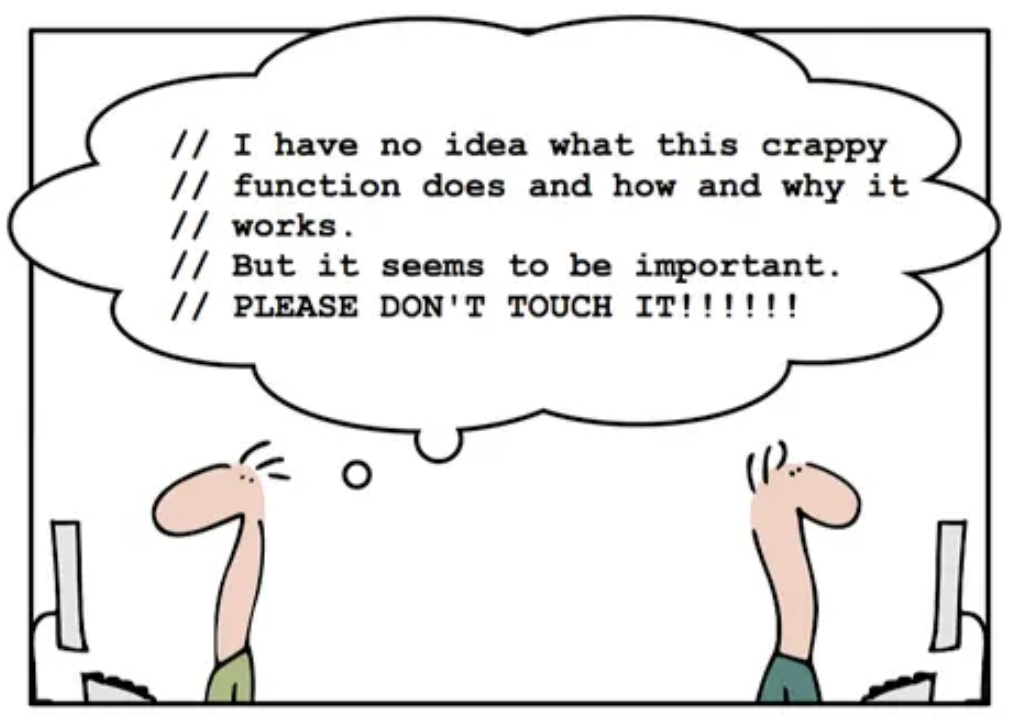
\includegraphics[width=.9\linewidth]{joke.png}
\source{spertus2021}
\end{multicols}}

\pitch{\pptBanner{Some Open Source Repositories (9 Feb 2024)}
{\ttfamily\small\begin{tabular}{llrrrr}
\toprule
Github Repository & Stack & Files & Comments & LoC & Com/LoC \\
\midrule
\href{https://github.com/nodejs/node}{nodejs} & JS \& C++ & 32559 & 1003K & 8381K & 0.12 \\
\href{https://github.com/pytorch/pytorch}{pytorch} & Python & 11562 & 414K & 2527K & 0.16 \\
\href{https://github.com/moby/moby}{moby} (a.k.a. Docker) & Go & 8389 & 272K & 1685K & 0.16 \\
\href{https://github.com/flutter/flutter}{flutter} & Dart & 5517 & 244K & 1353K & 0.18 \\
\href{https://github.com/spring-projects/spring-framework}{spring-framework} & Java & 9883 & 400K & 880K & 0.45 \\
\href{https://github.com/google/guava}{guava} & Java & 1984 & 131K & 479K & 0.27 \\
\bottomrule
\end{tabular}}}

\pitch{\pptBanner{My Own Statistics (9 Feb 2024)}
{\ttfamily\small\begin{tabular}{llrrr}
\toprule
Github Repository & Stack & Comments & LoC & Com/LoC \\
\midrule
\href{https://github.com/zerocracy/farm}{zerocracy/farm} & Java & 34380 & 58330 & 0.59 \\
\href{https://github.com/objectionary/eo}{objectionary/eo} & Java & 23383 & 49151 & 0.48 \\
\href{https://github.com/yegor256/cactoos}{yegor256/cactoos} & Java & 25857 & 33826 & 0.76 \\
\href{https://github.com/yegor256/takes}{yegor256/takes} & Java & 21393 & 26769 & 0.80 \\
\href{https://github.com/zold-io/zold}{zold-io/zold} & Ruby & 4306 & 11807 & 0.36 \\
\href{https://github.com/yegor256/tacit}{yegor256/tacit} & CSS & 259 & 1110 & 0.23 \\
\bottomrule
\end{tabular}}\par
All repositories are open source.}

\end{document}
